\documentclass[10pt,oneside,swedish]{lips}

%\usepackage[square]{natbib}\bibliographystyle{plainnat}\setcitestyle{numbers}
%\usepackage[round]{natbib}
\bibliographystyle{IEEEtran}

% Configure the document
\title{Designspecifikation}
\author{Projektgrupp 13}
\date{1 november 2022}
\version{1.0}

\reviewed{Hannes Nörager}{2022-11-01}
\approved{ }{ }

\begin{document}
\projecttitle{Taxibil-robot}

\groupname{Projektgrupp 13}
\groupemail{TSEA29_2022HT_E7-Grupp13@groups.liu.se}
\groupwww{https://gitlab.liu.se/da-proj/microcomputer-project-laboratory-d/2022/g13}

\coursecode{TSEA29}
\coursename{Konstruktion med mikrodatorer}

\orderer{Anders Nilsson, ISY, Linköpings universitet}
\ordererphone{013-28 26 35}
\ordereremail{anders.p.nilsson@liu.se}

\customer{Anders Nilsson, ISY, Linköpings universitet}
\customerphone{013-28 26 35}
\customeremail{anders.p.nilsson@liu.se}

\courseresponsible{Anders Nilsson, ISY, Linköpings universitetn}
\courseresponsiblephone{013-28 26 35}
\courseresponsibleemail{anders.p.nilsson@liu.se}

\supervisor{Peter Johansson}
\supervisorphone{013-28 1345}
\supervisoremail{peter.a.johansson@liu.se}

\smalllogo{../Figures/LiU_primary_black} % Page header logo, filename
\biglogo{../Figures/logo} % Front page logo, filename

\cfoot{\thepage}
\begin{document}
\maketitle

\cleardoublepage
\makeprojectid

\begin{center}
  \Large Projektdeltagare
\end{center}
\begin{center}
  \begin{tabular}{|l|l|l|l|}
    \hline
    \textbf{Namn} & \textbf{Ansvar} & \textbf{Telefon} & \textbf{E-post}\\
    \hline
    Linus Thorsell & Projektledare & 0765612171 & linth181@student.liu.se\\
    \hline
    Oscar Sandell & Testansvarig & 0709416866 & oscsa604@student.liu.se\\
    \hline
    Hannes Nöranger & Utvecklare & 0733118779 & hanno696@student.liu.se\\
    \hline
    Johan Klasén & Dokumentansvarig & 0730982555 & johkl473@student.liu.se\\
    \hline
    Zackarias Wadströmer & Utvecklare & 0706142029 & zacwa923@student.liu.se\\
    \hline
    Thomas Pilotti Wiger & Konstruktionsansvarig & 0761708593 & thopi836@student.liu.se\\
    \hline
  \end{tabular}
\end{center}


\cleardoublepage
\tableofcontents

\cleardoublepage
\section*{Dokumenthistorik}
\begin{tabular}{p{.06\textwidth}|p{.1\textwidth}|p{.33\textwidth}|p{.20\textwidth}|p{.20\textwidth}} 
  \multicolumn{1}{c}{\bfseries Version} & 
  \multicolumn{1}{|c}{\bfseries Datum} & 
  \multicolumn{1}{|c}{\bfseries Utförda förändringar} & 
  \multicolumn{1}{|c}{\bfseries Utförda av} & 
  \multicolumn{1}{|c}{\bfseries Granskad}\\
  \hline
  \hline
  0.1 & 2022-10-05 & Första utkast & Gruppen & Zackarias Wadströmer   \\
  \hline
  0.2 & 2022-10-13 & Andra utkast & Gruppen & Johan Klasén   \\
  \hline
  1.0 & 2022-11-01 & Första Versionen & Gruppen & Hannes Nörager   \\
  \hline
\end{tabular}

\cleardoublepage
\pagenumbering{arabic}\cfoot{\thepage}

\section{Inledning}
Det system som beskrivs i detta dokument har i uppdrag att agera autonom taxibil. Taxibilen har i uppdrag att hämta upp en passagerare vid en viss punkt för att sedan åka till en annan punkt där passageraren ska avlämnas. Systemet i fråga består av fyra olika delsystem; Kommunikationsmodul, Styrmodul, Sensormodul och en även en Extern Applikation.


\section{Översikt av systemet}

\begin{figure}[htbp]
  \centering
  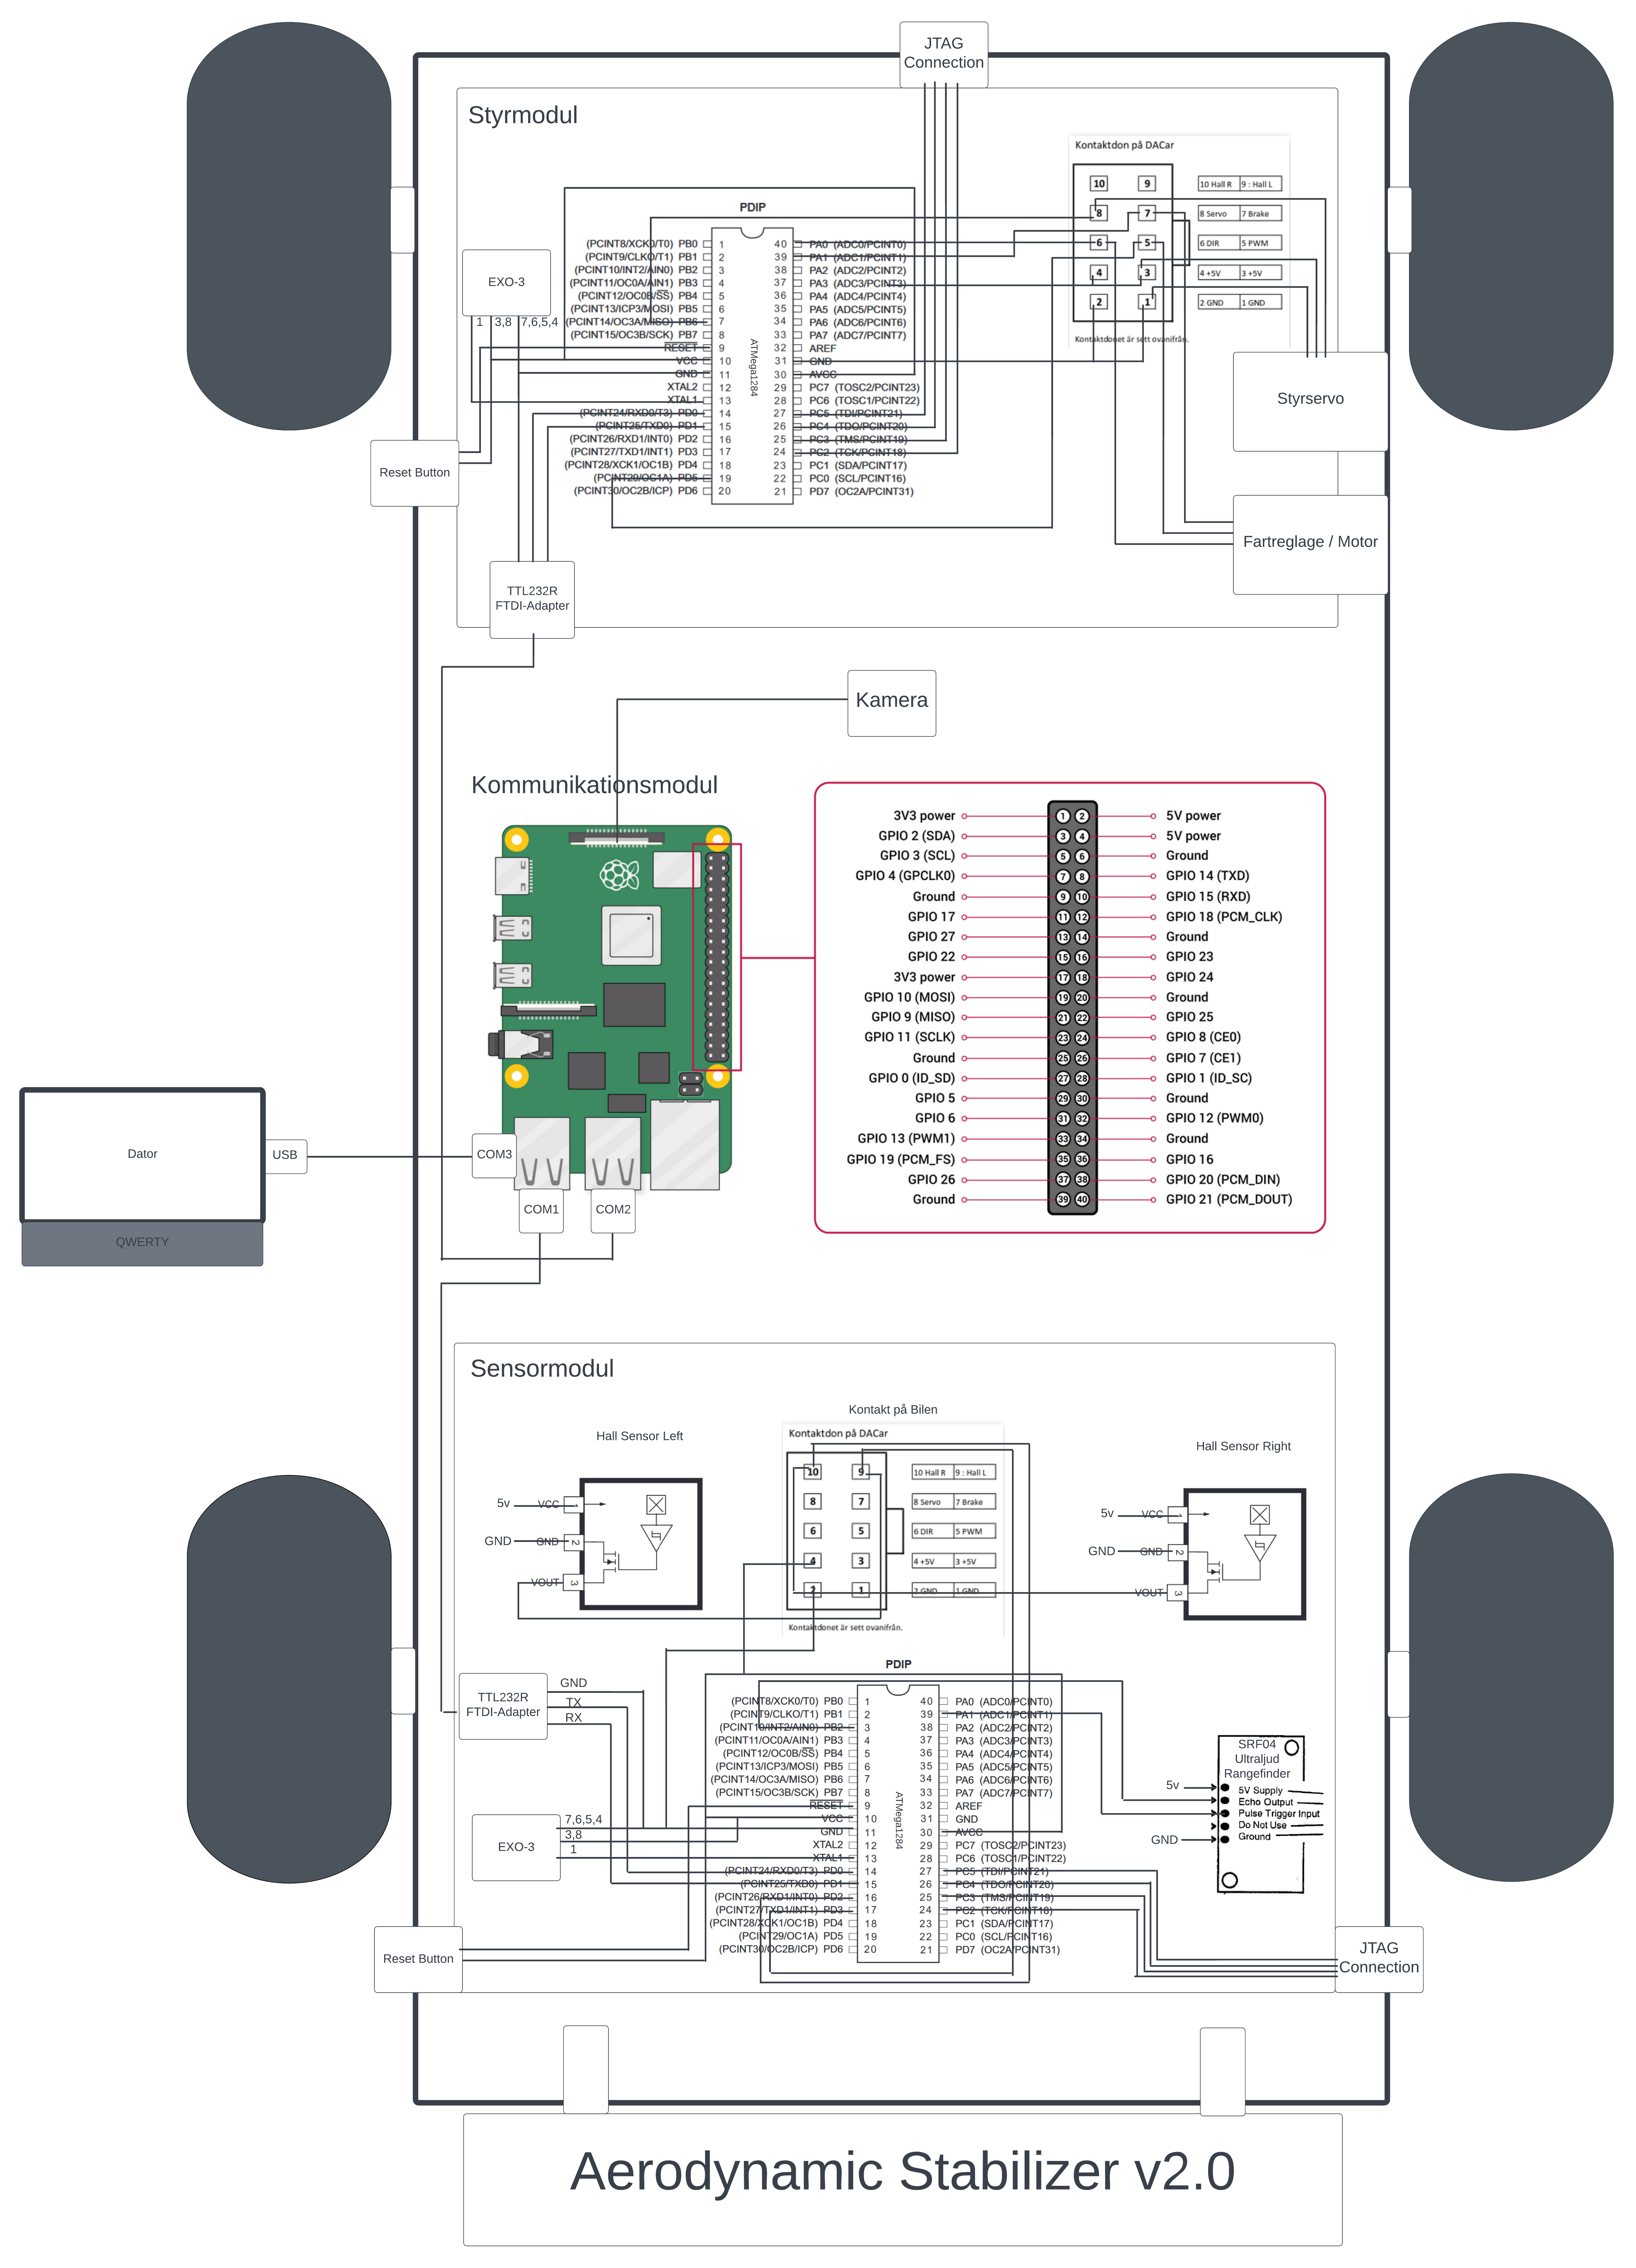
\includegraphics[width=.6\textwidth]{./Figures/detalj_oversikt.png}
  \caption{Övergripande blockschema över systemet som ska konstrueras.}https://www.overleaf.com/project/6328331fd6cd43a87f835da1
  \label{fig:detalj_oversikt}
\end{figure}
\clearpage

I figur \ref{fig:detalj_oversikt} syns ett övergripande blockschema över systemet som ska konstrueras. Den visar de fyra delsystemen \emph{kommunikations-, styr-} och \emph{sensormodulerna} samt den \emph{externa applikationen}, i bilden benämnd ``Webapp``. I centrum står kommuikationsmodulen som är det enda delsystem som är anslutet direkt till dem andra delsystemen. All data som behöver nå en annan modul går alltid via kommunikationsmodulen först om datan inte redan kommer därifrån.
Kommunikationsmodulen är ansluten till både sensor- och styr-modulen via \emph{UART}-protokoll och till webappen via WiFi. De tre modulerna ska alla kunna bytas ut mot en annan modul som följer samma implemtationsspecifikation, även om projektet endast innefattar utvecklingen av en av varje modul. 

% Blockschema, identifiera delsystem och
% gränssnitt, modularitet och uppgraderbarhet

\section{Delsystem 1: Kommunikationsmodul}

\begin{figure}[htbp]
  \centering
  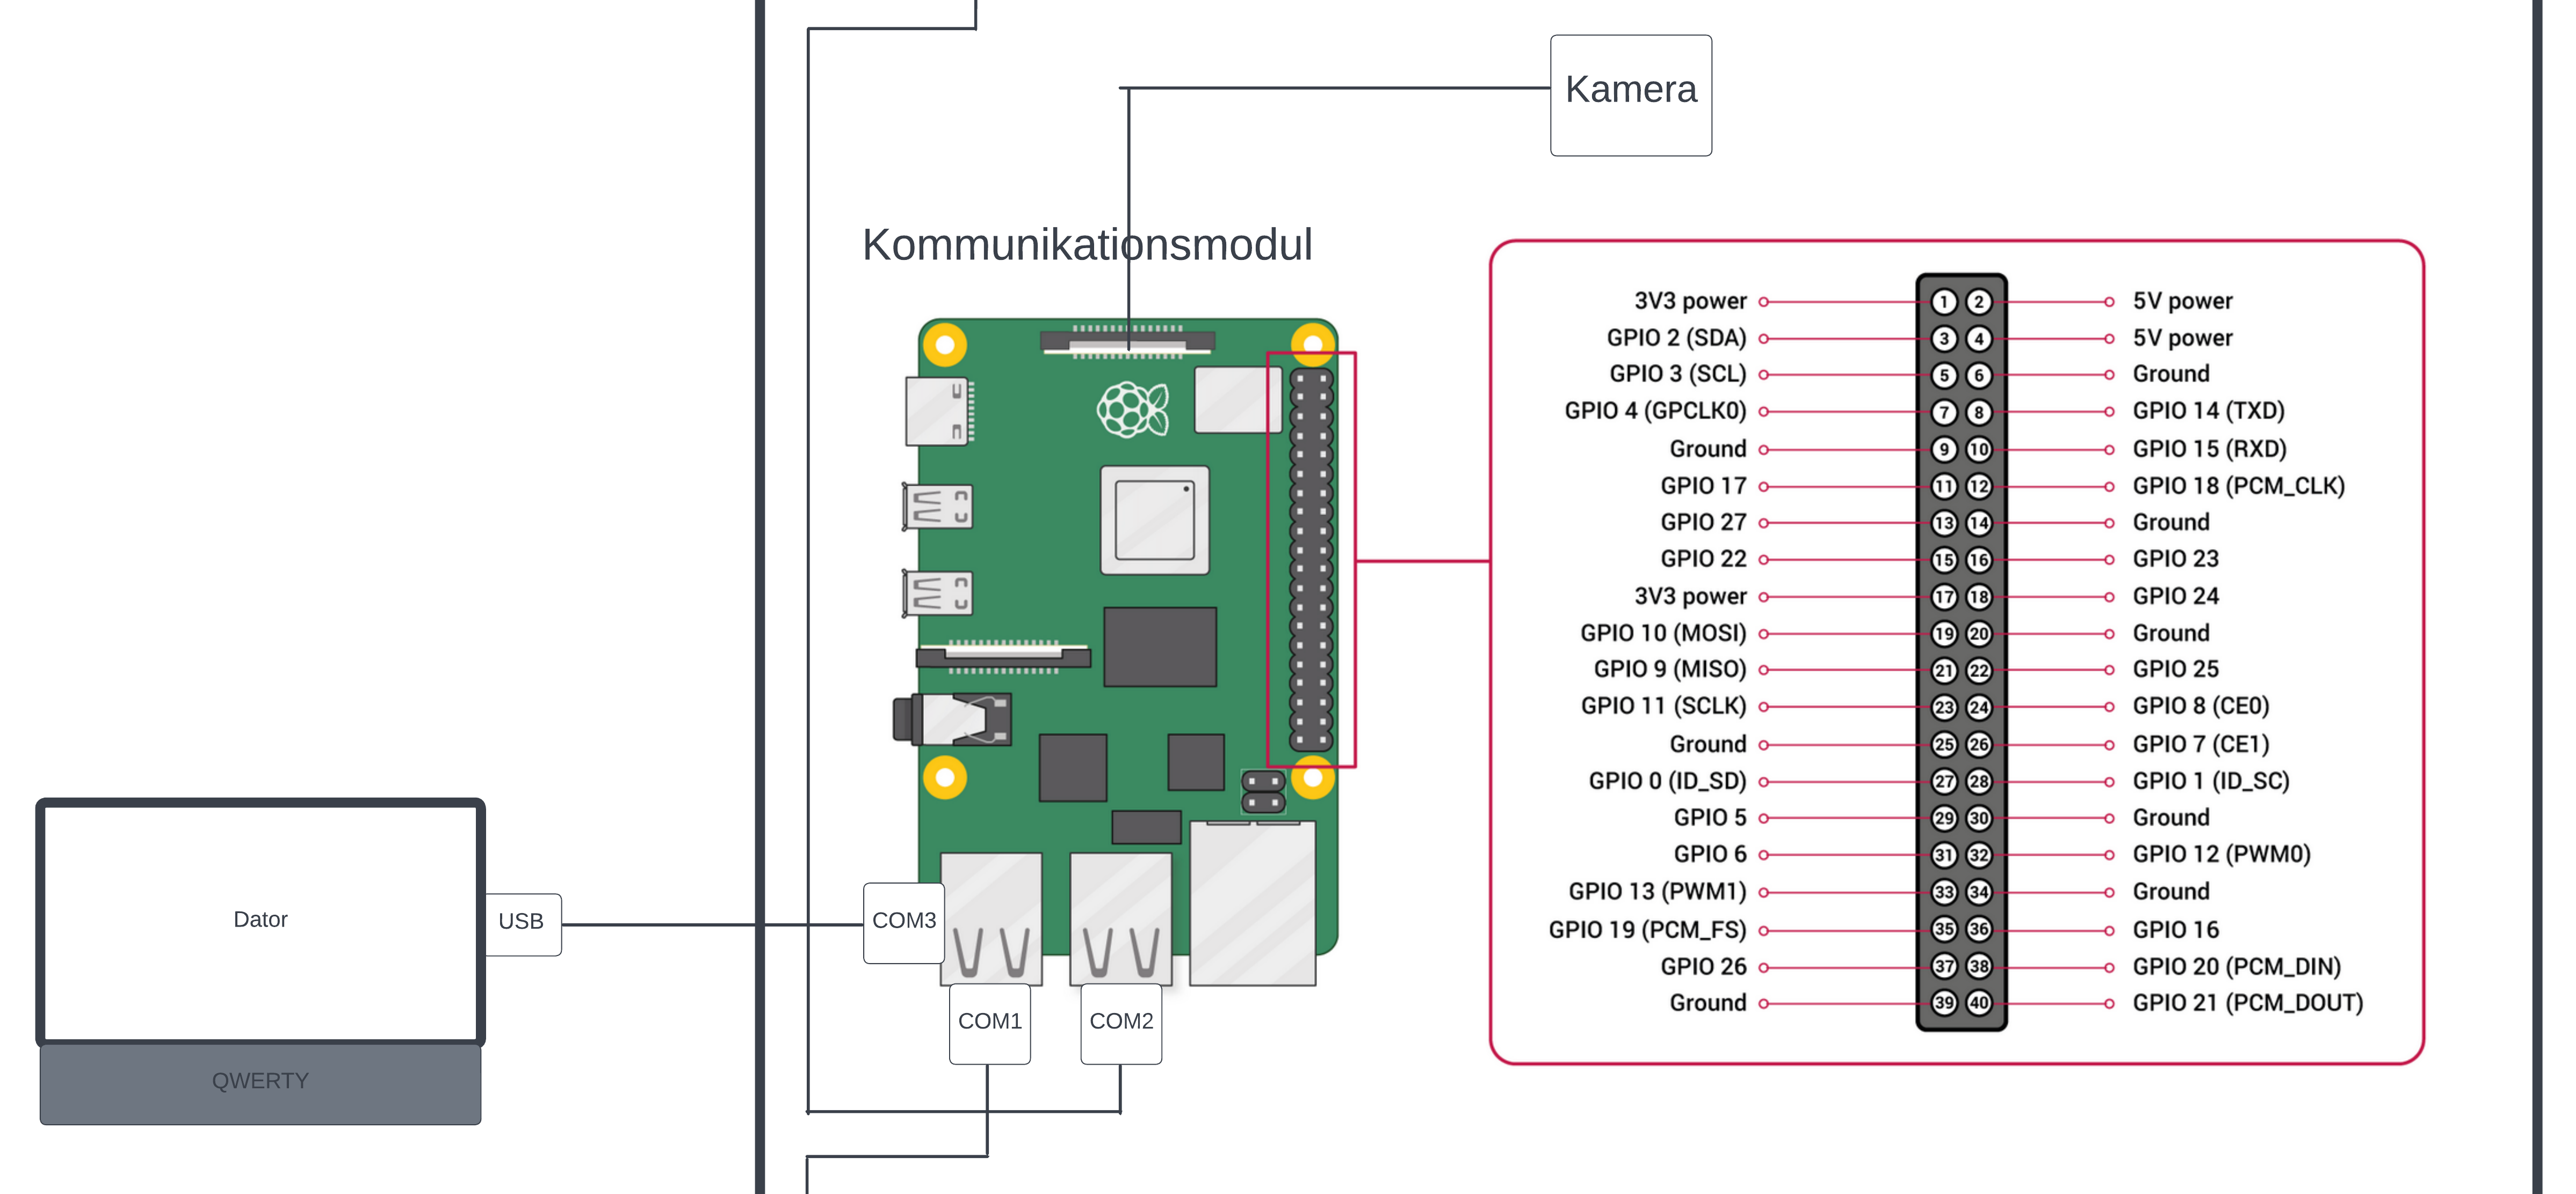
\includegraphics[width=1\textwidth]{./Figures/detalj_kommunikationsmodul.png}
  \caption{Övergripande blockschema över kommunikationsmodulen.}
  \label{fig:detalj_kommunikationsmodul.png}
\end{figure}

Kommunikationsmodulen består av en Raspberry-pi 3B+ och en Raspberry-pi-kamera. Denna modul ansvarar för ett antal saker, för det första är modulen ansvarig för att bearbeta data som tas emot från kameran och skicka vidare till styrmodulen. 
Kommunikationsmodulen fungerar också som en brygga mellan sensormodulen och styrmodulen, den tar emot data från sensormodulen och skickar vidare till styrmodulen.
Utöver de ovan nämnda funktionerna skickar kommunikationsmodulen all tillgänglig data till en extern dator. Kommunikationsmodulen kan också ta emot kommandon från en extern enhet och vidarebefordra dessa till styrmodulen.


\begin{figure}[htbp]
  \centering
  \includegraphics[width=0.92\textwidth]{./Figures/Kommunikationsmodul-Process.jpg}
  \caption{Skiss på idé på hur processen i kommuikationsmodulen kan se ut. Streckad funktionalitet är önskat men inte krävt. Int är förkortning för interrupt och motsvarar subrutiner eller parallella processer som körs vid sidan av huvud processen.}
  \label{fig:kommunikationsmodul-process}
\end{figure}

\pagebreak
\subsection{Sensor, Kamera}
En Raspberry-pi-kameran kommer att vara inkopplat direkt till Raspberry-pi för den att hantera indatan internt i. Kameran kan producera olika video format med bildfrekvenser för just dem formaten som finns i tabell \ref{tab:KameraBild}. Exakt vilket videoformat som används beslutas först när behovet av bildkvalité och frekvens blir uppenbart. 

\begin{table}[htpb]
    \centering
    \caption{Olika videoformat för Raspberry-pi kamera modul v2}
    \label{tab:KameraBild}
    \begin{tabular}{|l|l|}
    \hline
      {\bfseries Video format } & 
      {\bfseries Frekvens}  \\
      \hline
      1080 & 30 \\
      \hline
      720 & 60 \\
      \hline
      640x480 & 60/90 \\
      \hline
    \end{tabular}
\end{table}

\subsection{Navigatör}
Navigatören är funktionaliteten i kommunikationsmodulen som ansvarar för att minnas vart bilen är på banan och vad för beslut som den måste ta för att nå sitt mål snabbast, samt om den ska stanna vid nästa stopp. Navigatören tar emot data från den externa applikationen för att konstruera en datastruktur som beskriver banan innan start och använder denna genom körningen.

\subsection{Datorseende}
För att taxibilen ska kunna navigera sig genom banan kommer den använda sig av kamerasensorn i kommunikationsmodulen. I den modulen behandlas bilden för att producera styrdata till styrmodulen. Datorseendet kommer att hanteras med hjälp av biblioteket \emph{''OpenCV''} vilket kommer att installeras på Raspberry-Pi. 
Bilden från kameran kommer att skalas och filtreras för att bli hanterbart och sedan tolkas med hjälp av \emph{''OpenCV''} för att identifiera vägbana, stopp och korsningar. Den filtrerade bilden  kommer att skickas till den externa applikationen för att visas upp. 
Tolkningen om vad som finns framför bilen kommer att beaktas i samband med informationen från navigatören för att producera korrekt styrdata. Från bilden ska även felet från centrum av vägen räknas ut samt graderna mellan bilen och vägen. 
Den producerade styrdatan kommer att bestå av avstånd till stopplinje, avstånd från vägens centrum och vinkelfel vilket alla kommer att skickas till styrmodulen. Avstånden kommer att vara i centimeter och vinkelfel i grader (negativa grader för vänster, positiva för höger, 0 för mitten).

\begin{figure}[htbp]
  \centering
  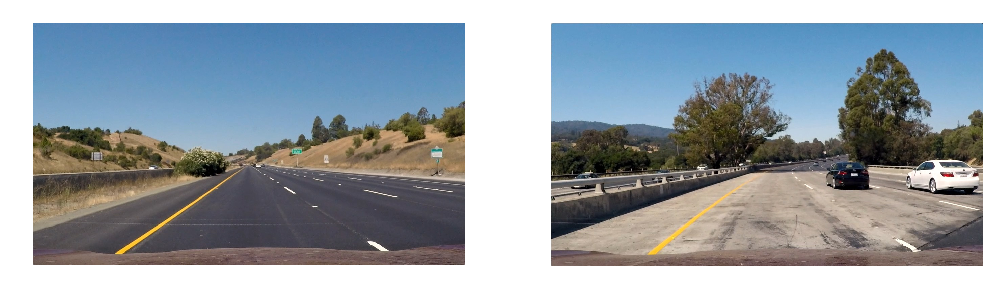
\includegraphics[width=0.7\textwidth]{./Figures/datorseende_normal.png}
  \caption{En exempel bild på en väg med två linjer att följa. Anpassad från \cite{Moataz} }
  \label{fig:datorseende_normal.png}
\end{figure}

\begin{figure}[htbp]
  \centering
  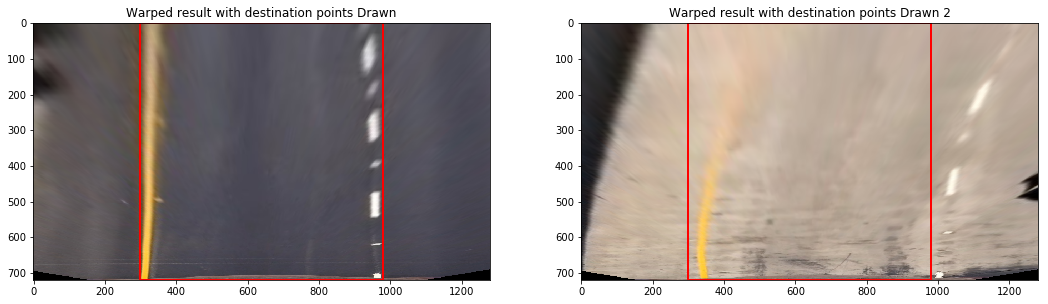
\includegraphics[width=0.7\textwidth]{./Figures/datorseende_filtrering.png}
  \caption{Detta är ett exempel på filtrerade bilder av dem från figur \ref{fig:datorseende_normal.png}. Den har plattats ut så att perspektiv och linsböjning är borttaget och endast det område av intresse, vägen, är på bilden. Hämtad från \cite{Moataz} }
  \label{fig:datorseende_filtrering.png}
\end{figure}

\begin{figure}[htbp]
  \centering
  \includegraphics[width=0.7\textwidth]{./Figures/datorseende_uträkning.png}
  \caption{Exempel på hur uträkningen kan se ut på bilderna från figur \ref{fig:datorseende_filtrering.png}. Uträkningarna kommer att hitta linjerna på bilden och markera dem för att sedan lista ut böjning och placering av dessa i förhållande med bilen. Hämtad från \cite{Moataz} }
  \label{fig:datorseende_uträkning.png}
    
\end{figure}





\pagebreak
\section{Delsystem 2: Styrmodul}
Styrmodulen består av en ATmega1284-processor. Denna processor har i uppdrag att kontrollera systemets motorer och servon, via koppling till ett kontaktdon i bilens skelett. Motorstyrningen sker via pulsmodulering där pulsbredden avgör hastighet respektive styrvinkel. 

\begin{figure}[htbp]
  \centering
  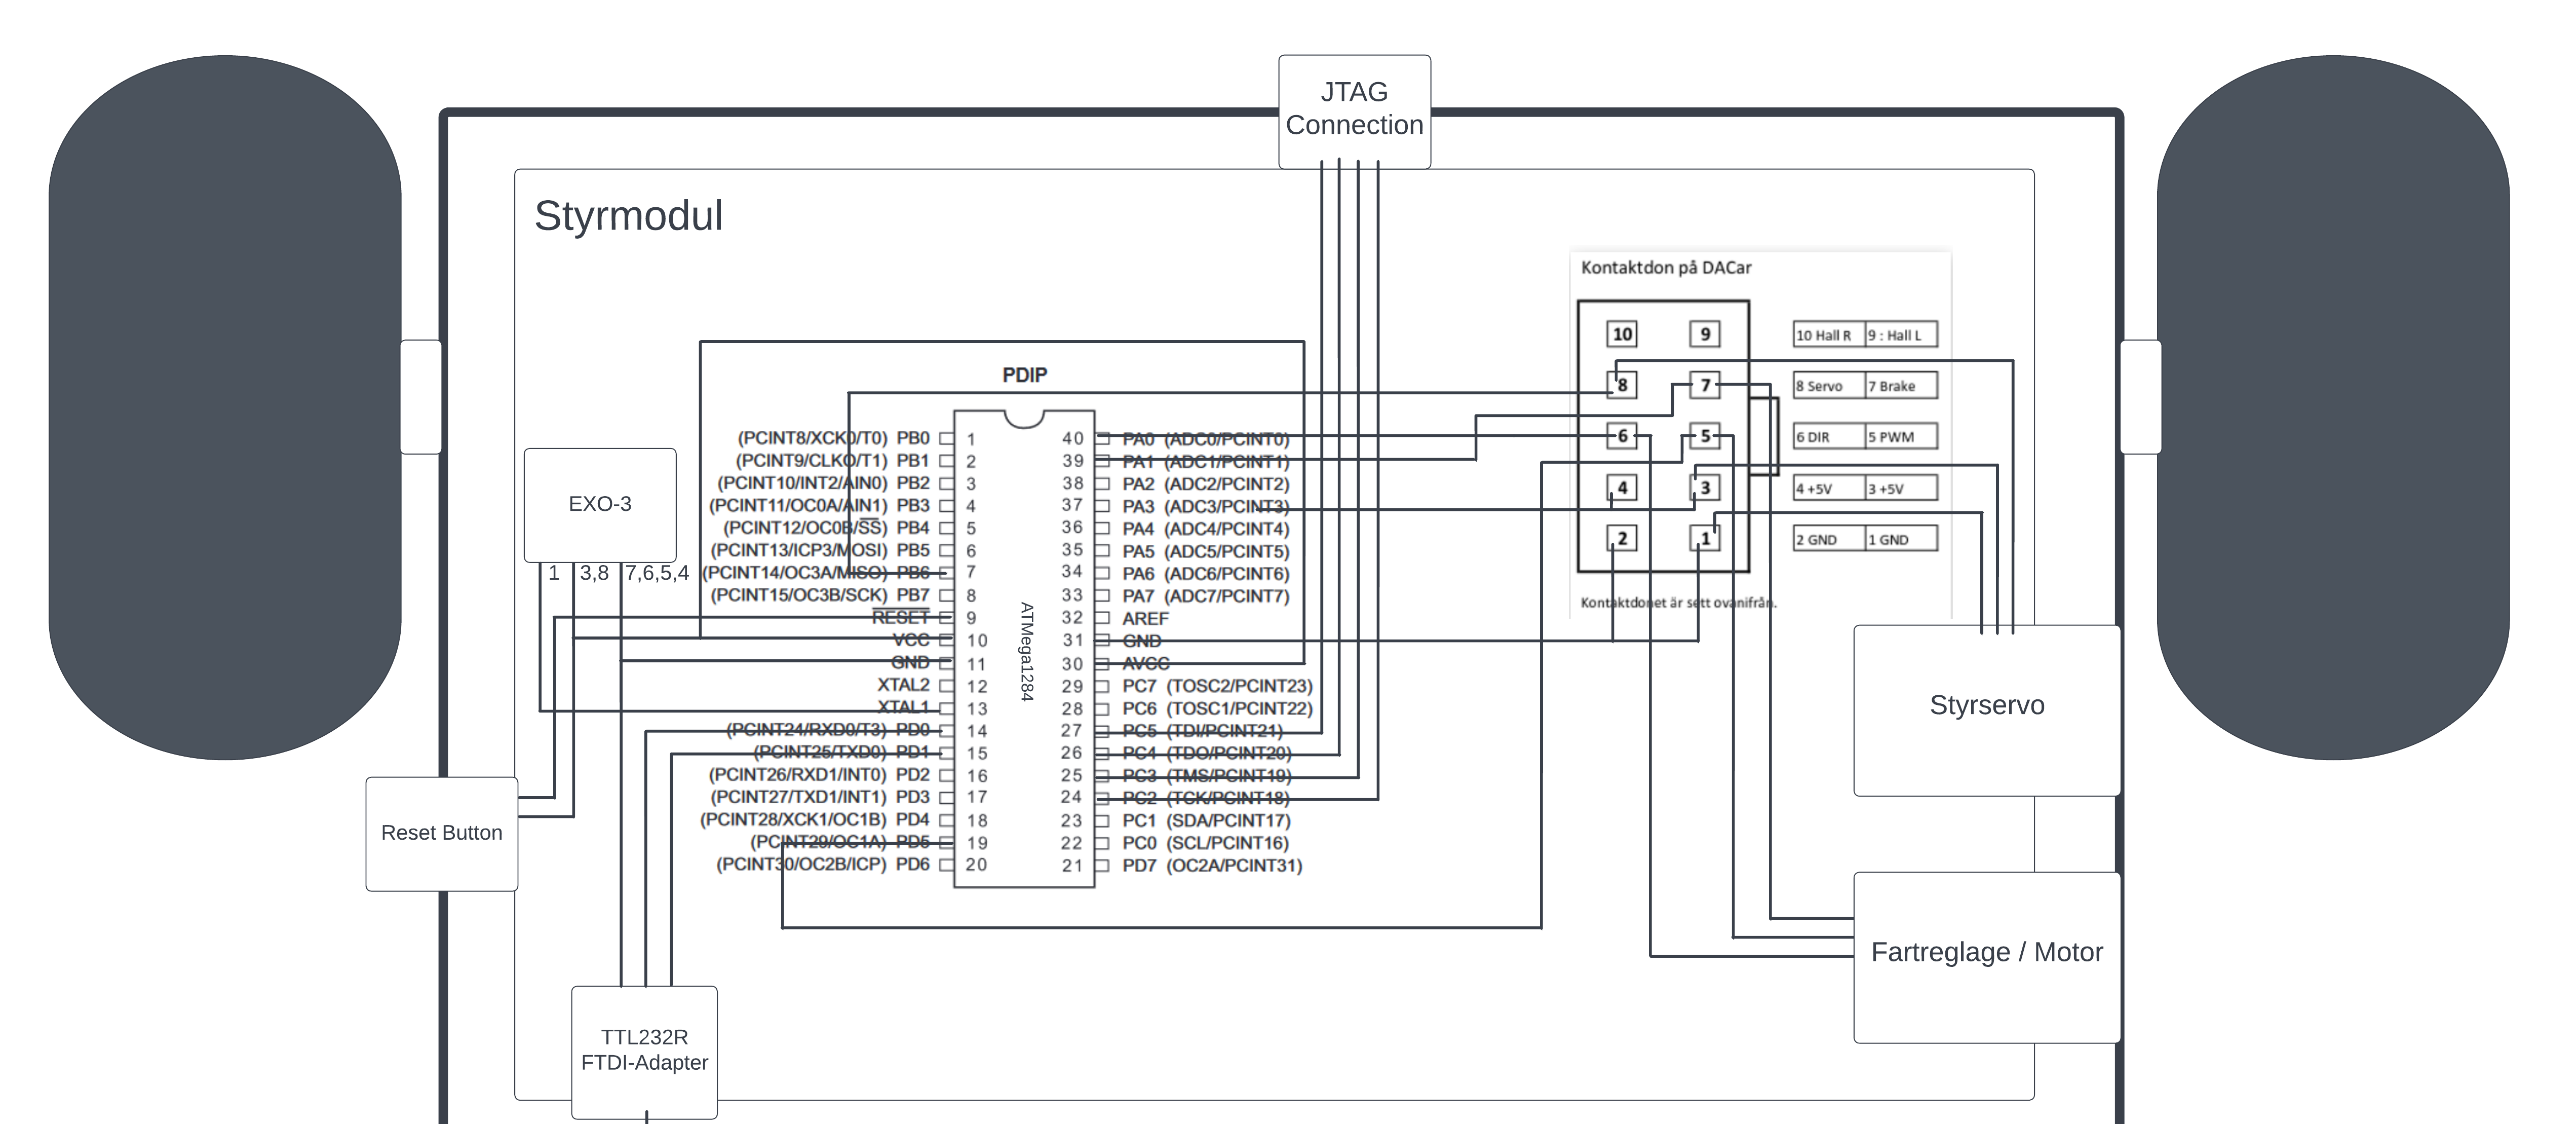
\includegraphics[width=1\textwidth]{./Figures/detalj_styrmodul.png}
  \caption{Övergripande blockschema över styrmodulen.}
  \label{fig:detalj_styrmodul.png}
\end{figure}

Modulen tar emot indata från kommunikationsmodulen i form av manuella kommandon, styrinformation för autonom körning i form av ett vinkelfel och avstånd till stopplinjer, samt tolkad sensordata i form av avstånd till fysiska hinder som kommer från ultraljudssensorn (se sektion \ref{sec:ultraljud} om sensorn). 
De manuella kommandona är förprogrammerade rutiner för att åka framåt, bakåt, höger, vänster eller stanna. 
Styrinformation används för att räkna ut hur bilen ska gasa, bromsa eller svänga för att hålla sig på banan, detta via en hastighetsloop och en PD-loop. Hastighetsloopen kontrollerar bilens hastighet och är beroende både av det avståndet till stopplinjer och vinkelfelet som ges i styrinformationen. Avståndet ska hjälpa till att avgöra när bilen nått sitt mål och ska stanna och vinkelfelet ska minimera risken för en s.k overshoot genom att få bilen att köra långsammare när vinkelfelet är väldigt stort.

\begin{figure}[htbp]
  \centering
  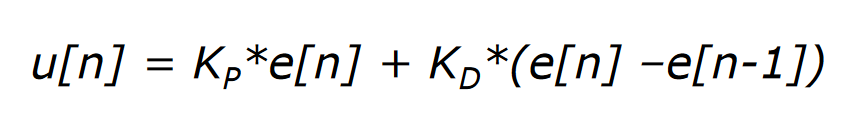
\includegraphics[width=0.35\textwidth]{./Figures/PD_formula.png}
  \caption{Ursprunglig formel för PD-reglering}
  \label{fig:PD.png}
\end{figure}

PD-loopen använder sig av nuvarande samt tidigare vinkelfel för att beräkna hur mycket bilen ska svänga för att nå ideal position (mitt emellan linjerna). Beräkningen görs enligt formeln som visas i figur \ref{fig:PD.png} där \textit{e} är ett invärde vid tid \textit{n}, \textit{u} utvärde och \textit{K} konstanter för termerna. Utvärdet omvandlas sedan till en PWM-signal som skickas till styrservot och ger ett styrutslag. Styrutslaget kommer påverka bilens position i vägbanan och ge upphop till ett nytt vinkelfel i bildbehandlingen. När det nya vinkelfelet har tagits emot från kommunikationsmodulen används det i nästa iteration av loopen.
Datan från ultraljudssensorn används för att avgöra när inbromsning för hinder ska ske och åsidosätter den autonoma körningen.
\clearpage


\section{Delsystem 3: Sensormodul}
Sensormodulen består av en ATmega-1284 processor, en ultraljudsensor och 2 halleffektssensorer. ATmega-1284 processorn används för att samla data från ultraljudssensorn och Hallefektsensorn, båda via interrupts. Tolka datan och skicka vidare den till kommunikationsmodulen via UART.

\begin{figure}[htbp]
  \centering
  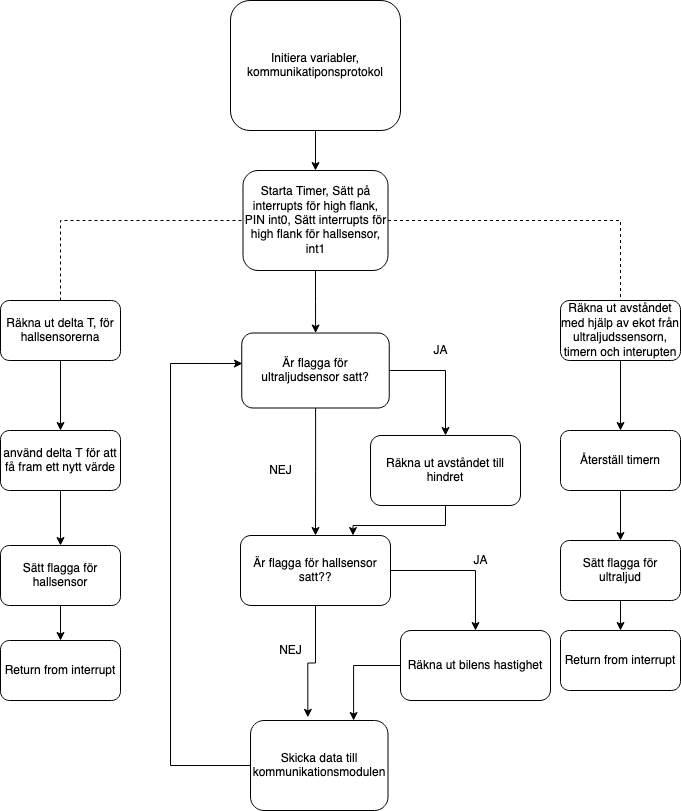
\includegraphics[width=.4\textwidth]{./Figures/SensormodulV2.drawio.png}
  \caption{Väldigt simpelt flowchart för koden i sensormodulen.}
  \label{fig:sensorflow}
\end{figure}

\subsection{Ultraljudssensor} \label{sec:ultraljud}
Ultraljudssensorn skickar ut en ultraljud-signal i en 45 grader bred kon och ger en hög signal för att visa sig redo att ta emot ett eko. Ekosignalen är hög tills ett eko uppfattats eller 36 ms förflutit (timeout). Längden till det objekt som signalen studsat mot kan då beräknas från bredden på ekosignalen i förhållande till ljudets hastighet (med en förmodad korrigering). Sensormodulen tittar på eko-signaler på en bredd som motsvarar 0.1-1 m.

\begin{figure}[htbp]
  \centering
  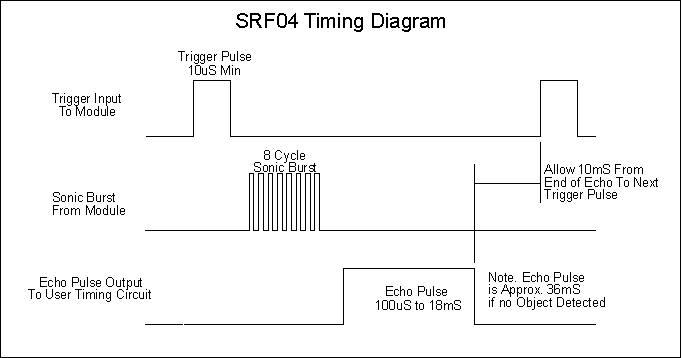
\includegraphics[width=.60\textwidth]{./Figures/srf04timing.png}
  \caption{Tidsdiagram för ultraljudsensorns signaler. \emph{Trigger Input} innebär starten av en mätning där sensorn svarar med att dra \emph{Echo Pulse Output} hög så fort den är redo att lyssna på ett eko och låg igen efter 36 ms (timeout) eller så fort ekot har tagits emot, vilket som kommer först.}
  \label{fig:us-timing}
\end{figure}

Ultraljudssenorns uppgift i systemet blir att fungera som en kollisionsdetektor och kommer sitta i framändan på bilen riktad i bilens körriktning. 
Ger sensorn utslag indikerar det att det finns något oväntat föremål på körbanan och man skickar då vidare avståndet till föremålet till styrmodulen så att den kan avgöra att den måste stanna,

\subsection{Halleffektssensor}
Vi använder en så kallad "switch" halleffektssensor, vilket betyder att den slår på när ett stort nog magnetfält påverkar den, och slår av när magnetfältet försvinner. Detta ger en 5 V signal när en magnet passerar och hastigheten tolkas från frekvensen av 5 V pulser.

Halleffektssenorerna sitter i anslutning till bilens båda bakhjul och på hjulen sitter tio magneter. Dessa magneter kommer få hallsensorerna att ge utslag när bilen är i rörelse och genom att räkna takten på utslagen och omkretsen på hjulen kan man räkna ut bilens hastigheten. 

\subsection{Data via UART}
Datan som skickas från sensormodulen ska vara genomsnittshastigheten (enhet kan anges senare när man vet ungefär hur snabbt den kör) och även avståndet till eventuella hinder i cm.


\begin{figure}[htbp]
  \centering
  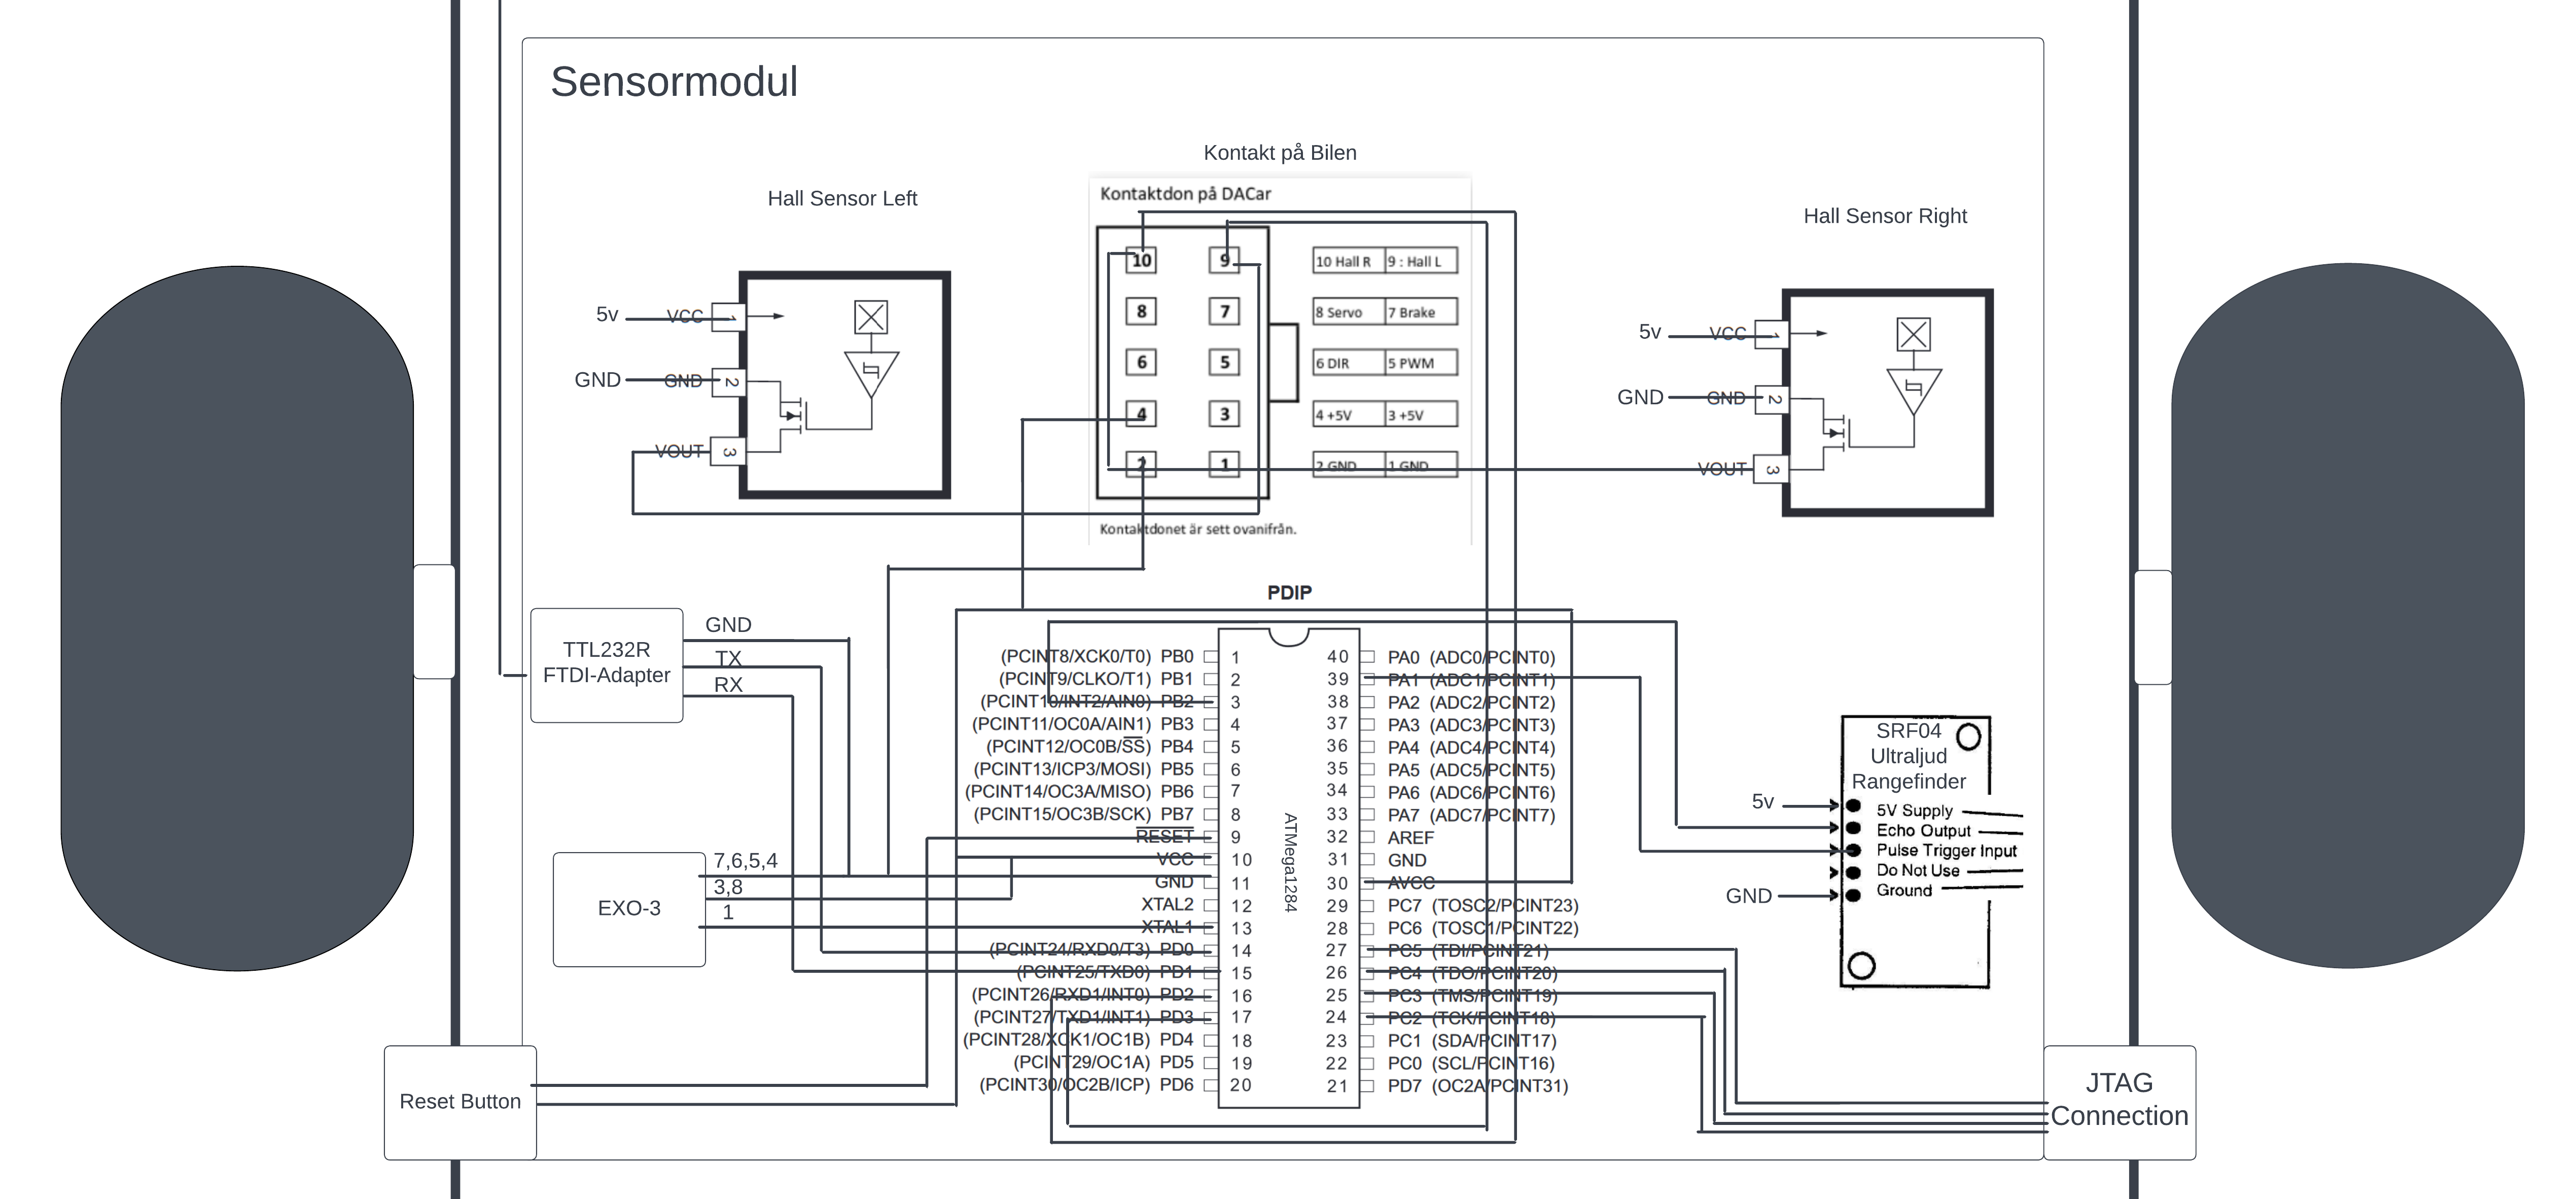
\includegraphics[width=0.92\textwidth]{./Figures/detalj_sensormodul.png}
  \caption{Väldigt enkel skiss på sensormodulen och de komponenter som är kopplade till den.}
  \label{fig:detalj_sensormodul.png}
\end{figure}

\clearpage

\section{Delsystem 4: Extern Applikation}
\begin{figure}[htbp]
  \centering
  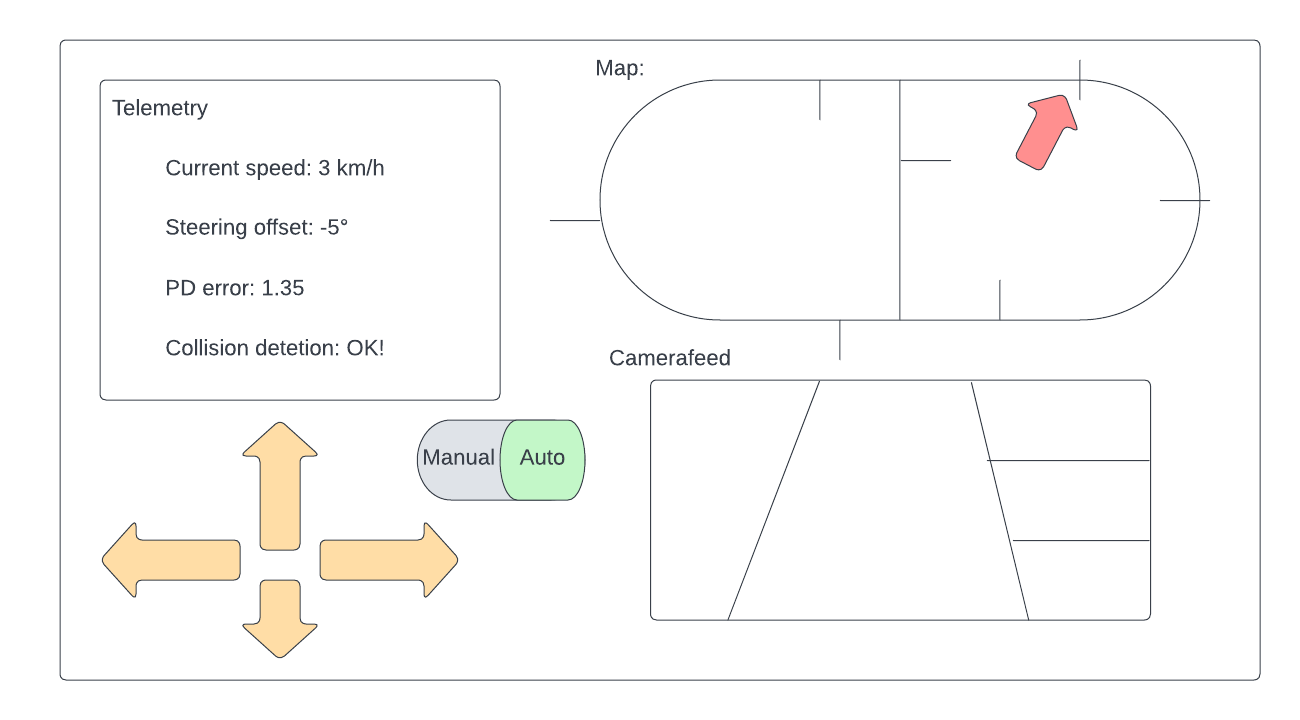
\includegraphics[width=.8\textwidth]{./Figures/appskiss.png}
  \caption{Väldigt enkel skiss på hur layouten på den externa applikationen skulle kunna se ut.}
  \label{fig:appskiss}
\end{figure}

Den Externa Applikationen består av en webserver som körs på en dator och kommunicerar telemetri och eventuellt en videoström mellan kommunikationsenheten och applikationen med hjälp av sockets i ett P2P förhållande, där servern är datorn och Raspberry-Pi'n är klienten. Telemetrin består av styrparametrar, som då kan ändra hur bilen beter sig på banan.

Figur \ref{fig:appskiss} visar ett exempel på hur layouten på applikationen skulle kunna se ut. Det finns fält med information om diverse styrparametrar och sensordata. Det finns möjlighet att växla mellan autonomt och manuellt styrläge och knappar eller på något annat vis möjlighet att skicka manuella styrkommandon till taxibilen. Vid sidan om kan man se en visualisering av banan med bilens position och en separat ruta som visar livebilder från kameran. Lämpligtvis finns det även möjlighet att ange och starta ett autonomt köruppdrag.

\section{Kommunikation mellan modulerna}

\subsection{Modulerna på taxin}
Både sensor- och styrmodulen kommunicerar med kommunikationsmodulen via UART protokollet och kommunikationsmodulen är i sin tur ansvarig för att föra vidare relevant information från sensormodulen till styrmodulen.

%Kommunikationen mellan sensorerna på taxibilen ska ske med hjälp av UART. Sensormodulen kommunicerar med komunikationsmodulen med hjälp av UART, kommunikationsmodulen kommunicerar med styrmodulen med hjälp av UART.
När sensor- och styrmodulen kommunicerar med kommunikationsmodulen så sker det med en simpel sträng. Strängen skulle kunna se ut såhär "\{D:45,V:5\}", där alla tecken är kodade med exempelvis ASCII. Där D är en etikett för avstånd i cm, V för velocity i km/h.
Det gör att man troligen behöver plocka ut delsträngar och göra en omvandling när man vill lägga in värdena i nummerära variabler, men gör att det väldigt lätt att utöka sändningen om man i senare skede inser att man behöver skicka mer data.

\subsection{Den Externa applikationen}
Kommunikationsmoudulen kommunicerar med den externa applikationen med hjälp av Wi-Fi då den externa applikationen är en webapp som Raspberry-Pi'n kopplar upp sig mot. Kommunikationen sker med hjälp av ett \emph{JSON}-format för informationsutbytet. Förhållandet mellan den externa applikationen och Raspberry-Pi'n är ett P2P förhållande.


\section{Komponentlista}
Utöver bilen och dator för extern applikation krävs:
\begin{itemize}
    \item Raspberry-pi 3B.
    \item Raspberry-pi Kamera v2 (160 graders lins).
    \item Ultraljudssensor, SRF04.
    \item Halleffektssensor, A1120.
    \item 2x Mikroprocessorer, ATmega1284P.
    \item 2x FTDI adapter, TTL232R.
    \item 2x Kristalloscillatorer, EXO-3 16MHz.
    \item 2x Reset-knappar.
    \item 2x Avstudsade knappar för testning av halleffektsensorer.
\end{itemize}

%\section{Utvecklingsmetodik}
%Standarder som gruppen kommer att efterleva i utvecklingen av %produkten.

\section{Implementeringsstrategi}
%\subsection{Test och integreringsstrategi}
\subsection{Konstruktionsmetodik}
När bilen utvecklas så ska det ske utifrån ''inifrån ut'', dvs att modulerna utvecklas i isolation för att sedan integreras till ett system.

\subsection{Programmeringsspråk}
Mjukvaran i Raspberry-Pi i kommunikationsmodulen kommer att programmeras genom \emph{''Python''}. Mikrodatorerna i sensormodulen och styrmodulen kommer att programmeras med \emph{''C/C++''}.

\subsection{Kontinuerlig Testning}
När modulerna utvecklas så kan det ske med kontinuerlig testning. Denna testning kan ske med en logikanalysator kopplade till modulerna. Man kan då använda sig utav en \emph{JTAG}-anslutning för att få en korrekt bild av vad som händer i processorn.

Ett annat sätt är att datan som skickas till kommunikationsmoudlen sparas i loggfiler så att man kan titta i loggfilen om något behöver debuggas.
% http://www.da.isy.liu.se/vanheden/pdf/DS_TTL-232R_CABLES.pdf
% TTL to USB Serial adapters, från Styr/Sensor-modul till raspberry-pins USB-portar. Dataöverföring via UART-protokoll. Beskriv vilken data som ska skickas i detta skede?
% Från Sensormodul: Hastighet? Snitt från båda sensorerna ? Ultraljud? Utslag av något gränsvärde

 \clearpage
\bibliography{references}



\end{document}